% REST playbook
\chapter{REST API Design}
\label{sec:ms}
Wie bereits zuvor erwähnt wurde, ist \ac{REST} \ac{API} kein industriell definierter Standard, weswegen es zahlreiche Varianten der Implementierung und Umsetzung gibt. Das Ziel dieses Kapitels ist es, allgemeingültige Richtlinien und Entwurfsstandards für die Erstellung einer \ac{REST}-\ac{API} der Hochschul-\ac{App} festzulegen. Diese Standards helfen beim genaueren Erarbeiten einer \acp{API}, die intuitiv ist und von den Entwicklern leicht verstanden und wieder- oder weiterverwendet werden kann.
\\
\linebreak

Eine \ac{REST}-\ac{API} kann in vier Bereiche aufgeteilt werden:

\begin{enumerate}
\item Ressourcen
\item Requests
\item Responses
\item Hypermedia
\end{enumerate}

Diese Bereiche werden in den kommenden Kapitel ausführlicher behandelt.

\section{Ressourcen Design}

Das folgende Kapitel betrifft Standards und Richtlinien für die Modellierung und Benennung von \ac{URI} Ressourcen, sowie für die Handhabung der HTTP-Methoden.

\subsection{Versionsverwaltung}

Die Versionierung ist ein wichtiger Aspekt des \ac{API}-Designs. Es kann jederzeit nachvollzogen werden, wann und was sich zu einer Version geändert hat - bei einem Problem kann das System auf eine vorherige Version wiederhergestellt werden. Somit soll jede \ac{API} einer Versionsnummer zugeordnet werden. Die Version kann aus einer Hauptversion und optional aus einer Nebenversion bestehen. Hierzu gibt es verschiedene Ansätze für die Versionsverwaltung. Es können bei verschiedenen Methoden, den Request-Parametern oder bei individuellen Headern die gewünschte Version angegeben werden. Zur Vereinfachung sollte das \ac{KISS}-Prinzip aus Kapitel \ref{sec:prinzipien} angewendet werden und die Version im Pfad der \ac{URI} mit dem Präfix \textit{v} und der Hauptversionsnummer angegeben werden. Bei folgenden Änderungen sollte die Version erhöht werden:

\begin{itemize}
\item Pflichtfeld wird als optional abgeändert oder umgekehrt
\item Pflichtfeld oder optionales Feld wird eingefügt
\item Ressourcen werden eingefügt, abgeändert oder entfernt
\item Datentypen werden hinzugefügt, geändert, entfernt oder eingeschränkt
\item Fehlercodes werden ergänzt
\end{itemize}

\subsection{URI Namenskonvention}

\ac{API}-\acp{URL} sollten folgende Kriterien enthalten:

\begin{itemize}
\item Adresse des Servers, auf dem die \ac{API} gehostet wird
\item Kennzeichnung, dass es sich um einen \ac{API}-Endpunkt handelt
\item Spezifizierung des \ac{API}-Namens
\item Spezifizierung der Version der \ac{API}
\item Spezifizierung der Ressource
\item Jede Pfadebene der Ressourcen muss sinnvolle Informationen liefern
\end{itemize}

Durch Beachtung dieser Kriterien sollte eine \ac{API}-\ac{URL} folgendermaßen aussehen:

\begin{lstlisting}[caption={URL Namenskonvention}, commentstyle=\color{black},]
http[s]://<server>/api/<api-name>/<api-version>/<resource>
https://hof-university.de/api/mensa-service/v1/menu
\end{lstlisting}

\subsection{Ressourcen Namenskonvention}

Folgende Namenskonventionen sollten für die Ressourcen in der Hochschul-\ac{App}-\ac{API} eingehalten werden:

\begin{itemize}
\item Jede Ressource muss einen aussagekräftigen und selbsterklärenden Namen haben. 
\item Wenn eine Ressource über Subressourcen verfügt, so werden diese durch Schrägstriche getrennt und der Pfad zur Subressourcen sollte hierarchisch und selbsterklärend aufgebaut werden.
\end{itemize}

Dies kann beispielsweise folgendermaßen aussehen:

\begin{lstlisting}[caption={Subressourcen Aufbau}]
/menu
/menu/{day}
/menu/{day}/{category}
\end{lstlisting}

Die Ressource \lstinline[columns=fixed]{/menu} soll %[]

\begin{itemize}

\item  alle verfügbaren Informationen zum \textit{Menü} liefern, 
\lstinline[columns=fixed]{/menu/today} nur für den heutigen Tag und \lstinline[columns=fixed]{/menu/today/desserts} nur für den heutigen Tag und nur für die Desserts,
\item keine \ac{CRUD} Operationsnamen in Ressourcen verwenden,
\item keine Mischung zwischen Groß- und Kleinschreibung enthalten,
\item keine Zeichen, die eine URL-Codierung erfordern, verwenden, 
\item Bindestrich anstelle eines Leerzeichens oder einer Unterstreichung verwenden.
\end{itemize}

\subsection{HTTP Methoden}
Nach der Identifizierung der Ressourcen für eine \ac{API} \footnote{Siehe Kapitel \ref{sec:appservices}}, muss die Aktion, die für diese Ressource ausgeführt werden soll, festgelegt werden. Dafür werden die HTTP-Methoden verwendet um die ausführende Aktion anzugeben. Die primären und am häufigsten verwendete HTTP-Methoden sind POST, GET, PUT und DELETE. 

\begin{figure}[H]
\centering
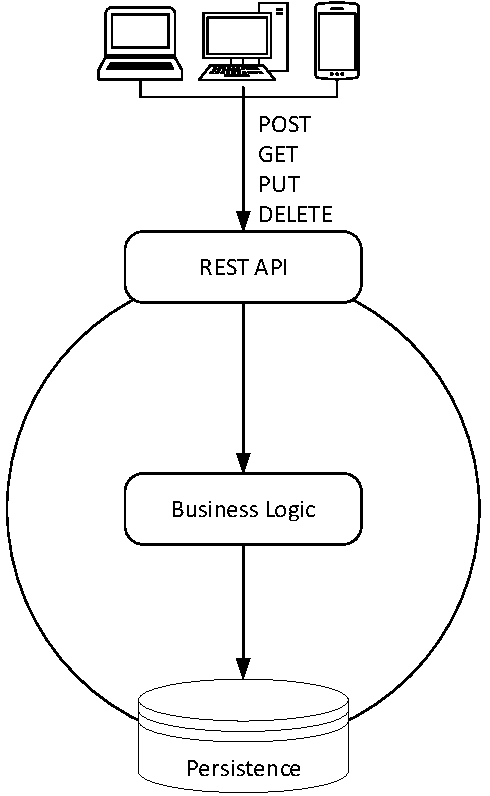
\includegraphics[width=\pictureWidth cm - 7.5 cm]{Bilder/Sonstiges/Rest_Api_HTTP.pdf}
\caption{Einordung der \ac{HTTP}-Methoden in  die Gesamtarchitektur\label{fig:api}\protect\footnotemark}
\end{figure}
\footnotetext{Brysiuk, Lehmann (2019)}


Diese Methode helfen bei der Ausführung der \ac{CRUD}-Operationen für die Ressource. Die Richtlinien für die Verwendung der Methoden in der Hochschul-\ac{App}-\ac{API} werden in Tabelle \ref{tab:httpmethoden} erläutert\autocite[Vgl.][]{httpwiki}.

\begin{table}[H]
\begin{center}
  \begin{tabular}{|  p{0.14\textwidth} |  p{0.8\textwidth} |}
  	\hline
  	\rowcolor{Gray}
  	\textcolor{white}{\textbf{Methoden}}			& \textcolor{white}{\textbf{Definition}} \\
    \hline
    GET		 									& Wird zum Abrufen oder Lesen der Informationen verwendet
    \\ \hline
    \rowcolor{LGray}
    POST									 		& Wird zum Erstellen einer neuen Ressource verwendet
    \\ \hline
    PUT									 		& Wird zum Aktualisieren/Änderung einer ganzen Ressource verwendet
    \\ \hline
    \rowcolor{LGray}
    DELETE								 		& Wird zum Löschen einer vorhandenen Ressource verwendet
    \\ \hline
    PATCH								 		& Wird zum Aktualisieren/Änderung eines teils einer Ressource verwendet
    \\ \hline
    \rowcolor{LGray}
    TRACE										& Wird zur Verfolgung von den Request verwendet
    \\ \hline
    OPTIONS								 		& Anforderung einer Liste vorhandenen HTTP-Methoden für diese Ressource
    \\ \hline
    \rowcolor{LGray}
    HEAD											& Ähnlich wie GET, jedoch wird nur der Response-Header zurückgegeben
    \\ \hline
    CONNECT										& Bereitstellung eines \ac{SSL}-Tunnels von Proxyservern %https://wiki.selfhtml.org/wiki/HTTP/Anfragemethoden
    \\ \hline
  \end{tabular}
  \end{center}
\caption[HTTP-Methoden]{Erläuterung der HTTP-Methoden}
\label{tab:httpmethoden}
\end{table}

Zudem kann die Methode \textit{TRACE} dazu dienen, die Requests auf Veränderungen während der Übertragung dieser zu überprüfen. \textit{HEAD} bietet unter anderem die Möglichkeit, die gecachten Daten auf Ihre Gültigkeit zur prüfen, ohne die ganzen Daten komplett neu anzufordern\autocite[Vgl.][]{httpwiki}.
%https://wiki.selfhtml.org/wiki/HTTP/Anfragemethoden

\section{Request Struktur}
\label{sec:reqstructure}

Das folgende Kapitel behandelt die Nachtrichten-Struktur-Richtlinien für Inhalt, Format, Header und Query Parameter einer Nachricht.

\subsection{Header}

Die folgende Liste enthält HTTP-Header, die von der Hochschul-\ac{App}-\acp{API} verwendet werden sollen:

\begin{itemize}
\item Accept
\item Authorization
\item Content-Type
\item X-HTTP-Method-Override
\end{itemize}

Das Payload-Format der Hochschul-\ac{App} wird nur auf das Format \ac{JSON} beschränkt, da \ac{JSON} einige Vorteile gegenüber anderen Formaten bietet, was in Kapitel \ref{sec:webservices} bereits erwähnt wurde. Mit dem Header \lstinline[columns=fixed]{accept} %[
kann der Medientyp des erwarteten Antwortinhalts und mit dem \lstinline[columns=fixed]{content-type} %[
der Medientyp des Requests angegeben werden. Also wird der \textit{Mediatype} als \lstinline[columns=fixed]{application/json} im \lstinline[columns=fixed]{content-type} und im \lstinline[columns=fixed]{accept} Header definiert. Der Header \lstinline[columns=fixed]{authorization} wird für die Benutzerauthentifizierung verwendet, der Header \lstinline[columns=fixed]{x-api-key} hingegen für die Clientauthentifizierung.%[

\subsection{Query Parameter}

Query Parameter sollten im allgemeinen möglichst vermieden werden. Zuerst soll immer versucht werden die Parameter als Subressourcen in der \ac{URI} hierarchisch aufzubauen. Dies erhöht die Lesbarkeit, Verständlichkeit, Flexibilität und reduziert die Komplexität der Ressourcen. Jedoch lässt es sich manchmal nicht vermeiden Query Parameter zu verwenden, meistens ist dies bei der Filterung oder Sortierungen der Ressourcen der Fall. Werden Query Parameter verwendet, soll folgendes beachtet werden:

\begin{itemize}
\item Query Parameter sollen sich nur auf die spezifizierte Ressource beziehen.
\item Komplexe oder aufwendige Query Parameter sollen im Request Body übergeben werden.
\end{itemize}

\subsection{Aufteilung einer Ressource}

Wenn eine Ressource eine große Menge von Ergebnissen zurückgeben kann, soll diese aus Performance gründen auf kleinere Teilmengen aufgeteilt werden. Folgende Richtlinien sollen bei Aufteilung einer Ressource beachtet werden:

\begin{itemize}
\item Die Größe der Teilmenge sollte auf einen Standardwert festgelegt werden.
\item Der Standardwert kann durch den Client geändert werden.
\item Das Ergebnis der Teilmenge sollten folgende Metadaten enthalten:
	\begin{itemize}
	\item Link zur ersten Seite
	\item Link zur vorherigen Seite, falls vorhanden
	\item Link zur aktuellen Seite
	\item Link zur nächsten Seite, falls vorhanden
	\item Link zur letzten Seite
	\item die Gesamtzahl der Teilmengen
	\end{itemize}
\item Die Seite der Teilmenge sollte mit dem Parameter \textit{offset} gekennzeichnet werden.
\item Der Parameter \textit{offset} und der Standardwert können als Query Parameter übergeben werden.
\end{itemize}

Eine mögliche Umsetzung dieser Richtlinien könnte folgend aussehen:
\newpage
\begin{lstlisting}[label=lst:teilmenge,caption={Aufteilung der Ressource Vorlesung}]
{ 
  links: {
    first: "/stundenplan-service/v1/lectures?offset=0,limit=50"
    prev:  "/stundenplan-service/v1/lectures?offset=1,limit=50"
    self:  "/stundenplan-service/v1/lectures?offset=2,limit=50"
    next:  "/stundenplan-service/v1/lectures?offset=3,limit=50"
    last:  "/stundenplan-service/v1/lectures?offset=23,limit=50"
  }
}
\end{lstlisting}

\section{Response Handling}

Im folgenden werden die Antworten behandelt, welche auf einen \ac{HTTP}-Request an den aufrufenden Client zurückgegeben werden. 

\subsection{Response Inhaltsformat}

Das Format von Antwortinhalten ist bei der Hochschul-\ac{App} auf \ac{JSON} beschränkt, wie bereits im Kapitel \ref{sec:reqstructure} erwähnt wurde. 

\subsection{HTTP Statuscode}

\ac{REST}-\acp{API} müssen Informationen zum Austausch mit den richtigen Statuscodes kommunizieren. Es gibt verscheiden Arten von Statuscodes, die Erfolgs- als auch Fehlerinformation mitteilen. Die Statuscodes können in vier Kategorien unterteilt werden:

\begin{itemize}
\item 2xx: Für Erfolgreiche Nachrichten
\item 3xx: Für Umleitungen
\item 4xx: Für Fehler Client-seitig
\item 5xx: Für Fehler Server-seitig
\end{itemize}

In Tabelle \ref{tab:status} sind die wichtigsten Statuscodes für die Hochschul-\ac{App} erläutert.
\newpage
  \begin{longtable}[c]{| p{0.055\textwidth} | p{0.28\textwidth} | p{0.58\textwidth} |}
  \hline
  \rowcolor{Gray}
  \textcolor{white}{\textbf{Code}} & \textcolor{white}{\textbf{Nachricht}} & \textcolor{white}{\textbf{Definition}} \\
   \hline
    200 &		  OK						& Die Anfrage war erfolgreich.
    \\ \hline
    \rowcolor{LGray}
    201	&		  Created				& Neue Ressource wurde erfolgreich angelegt.
    \\ \hline
    202	&		  Accepted				& Die Anfrage wurde erfolgreich angenommen, die Informationen über die tatsächliche Ausführung der Anfrage können nicht sofort zurückgesendet werden.
    \\ \hline
    \rowcolor{LGray}
    400	&		  Bad Request			& Fehlerhafte Anfrage des Clients.
    \\ \hline
    401	&		  Unauthorized			& Anfrage für diese Ressource benötigt Autorisierung.
	\\ \hline
	\rowcolor{LGray}
    403	&		  Forbidden				& Client hat keinen Zugriff auf die angeforderte Ressource.
    \\ \hline
    404	&		  Not Found				& Angefragte URI wurde vom Server nicht gefunden.
    \\ \hline
    \rowcolor{LGray}
    405	&		  Method Not Allowed		& Die Anfrage auf die Ressource ist nicht zulässig.
    \\ \hline
    409	&		  Conflict				& Die Anforderung konnte aufgrund eines Konflikts mit dem aktuellen Status der Ressource nicht verarbeitet werden.
    \\ \hline
    \rowcolor{LGray}
    414	&		  Request-URI Too Large	& Die Länge der angefragten \ac{URI} ist länger als das zulässige Limit für den Server.
    \\ \hline
    415	&		  Unsupported Media Type	& Angefordertes oder übergebenes Format wird vom Server nicht unterstützt.
	\\ \hline
	\rowcolor{LGray}
    429	&		  Too Many Requests		& Zu viele Anfragen wurden vom Client an die Ressource gestellt.
    \\ \hline
    500	&		  Internal Server Error	& Anfrage kann aufgrund eines unerwarteten Fehlers auf dem Server nicht verarbeitet werden.
    \\ \hline
    \rowcolor{LGray}
    503	&		  Service Unavailable	& Die Anfrage an den Service kann vorübergehen nicht verarbeitet werden.
    \\ \hline
\caption[HTTP-Statuscodes]{Erläuterung der HTTP-Statuscodes\label{tab:status}} 

  \end{longtable}

Außerdem ist die Übermittlung von richtigen Statuscodes zusätzlich mit einer Fehlernachricht für die gute Nutzbarkeit der \ac{API} von entscheidender Bedeutung. Durch gut definierte Statuscodes und Fehlernachrichten können Debugging und Fehlerbehebungen deutlich erleichtert werden, sowohl Client- als auch Server-seitig. Der Aufbau solcher Fehlernachrichten mit Statuscodes sieht folgendermaßen aus:

\begin{lstlisting}[caption={Aufbau Fehlernachricht}]
{
  status_code: {status},
  status_message: "status message",
  errors: [{
    error_code: {error code},
    error_message: "error message"
  }]
}
\end{lstlisting}

Eine \ac{API}, die mehrere Aufrufe an andere \acp{API} oder Systeme weiterleitet oder koordiniert, sollte einen einzelnen Statuscode zurückgeben, der das Ergebnis der kombinierten Ausführung von Aufrufen darstellt.

\subsection{Asynchrone Callbacks}

Es gibt zwei Standards für asynchrone Callbacks, entweder eine Callback-\ac{URL} oder eine Push-Notification. Bei einer Callback-\ac{URL} können die Clients eine \ac{URL} der \ac{API} zur Verfügung stellen, über welche die \ac{API} dem Client über Ergebnisse oder Ereignisse berichten kann. Bei Push-Notifications soll der Client über die Ereignisse informiert werden, auch wenn dieser gerade nicht aktiv auf dem Service ist. Der Standard von Push-Notifications für asynchrone Callbacks wird in der Hochschul-\ac{App} ebenfalls verwendet. Push-Notifications stellen eine gute Möglichkeit dar, die Studenten beispielsweise über Stundenplanänderungen in der Hoch\-schul-\ac{App} zu informieren. Weitere Informationen darüber sind im Kapitel \ref{sec:notification_api} zu finden.

\section{Hypermedia}

Die Technologie \ac{HATEOAS} ermöglicht es, eine \ac{API}-Ressource leichter auffindbar zu machen und erleichtert die Verwendung der \ac{API}-Ressourcen für den Benutzer. Dies wird dadurch ermöglicht, dass bei einem Request auf eine Ressource als Antwort Hyperlinks zu verwandten Ressourcen oder Endpunkten mit bereitgestellt werden. Für die Benutzer bedeutet das, dass keine Vorkenntnisse des Datenmodells oder Schemas erforderlich sind, um mit der \ac{API} navigieren und interagieren zu können. Wenn im Client bei der Implementation der Anwendung \ac{HATEOAS} berücksichtigt werden, werden die in der \ac{API}-Schnittstelle abgeänderten Ressourcen automatisch in der Client-Anwendung angepasst.
\\
\linebreak
Für die Vorteile von \ac{HATEOAS} in der Hochschul-\ac{App} kann folgende Situation betrachtet werden. Ein Benutzer der Hoch\-schul-\ac{App} kann sich einen personalisierten Stundenplan anlegen. Dieser Stundenplan wird in einem User-Service abgespeichert, wobei nicht alle Informationen zu den Vorlesungen gespeichert werden, sondern nur deren \acp{ID}. Bei der Darstellung des personalisierten Stundenplans im Client muss dieser zuerst eine Anfrage an den User-Service stellen und mit der erhaltenen Antwort eine neue Anfrage mit den \acp{ID} aufbauen und an Stundenplan-Service senden, um die Informationen der Vorlesungen zur erhalten. Durch die Verwendung von \ac{HATEOAS} stellt der Client eine Anfrage an den User-Service und in der Antwort ist ein Hyperlink enthalten, der bereits die Query für die benötigten \acp{ID} der Vorlesungen enthält.

\begin{lstlisting}[caption={HATEOAS Hyperlink}]
{
  links: {
    lectures: "/stundenplan-service/v1/lectures?ids=1,2,3"
  }
}
\end{lstlisting}

Der Client muss nur den Hyperlink aufrufen, ohne eine aufwändige Query zu erstellen, um Vorlesungsinformationen zu erhalten. Sollte sich die Ressource \lstinline[columns=fixed]{/lectures} %[
ändern, so hat das keine Auswirkung auf die Funktionalität des Clients, da die neue Ressource wieder als Hyperlink zur Verfügung steht. Die erwähnte User-Service Ausarbeitung ist in der parallel zu dieser Arbeit entwickelten Bachelorarbeit ausführlich beschrieben\autocite[Vgl.][]{andreasba}.
